\section{\sysname{} design}
\label{sec:generic}

The design of \sysname{} is driven by the need to address the three challenges
described in the previous section. Before delving into the details of the key
algorithms in \sysname{}, it is useful briefly describe the physical
implementation of \sysname{}. The implementation is described in detail in
\S\ref{sec:implementation}.

\sysname{} works by tagging packets.  A packet arrives at the ingress port $i$
of a switch $S$ with a tag $j$. The arriving packet packet is enqueued in queue
$j$.  At departure, based on the values of $i$ and $j$, the packet is possibly
given a new tag, say $k$. The rest of the forwarding pipeline, as well as PFC
PAUSE/Resume behavior (\S\ref{sec:background}) operates without change. 

The smartness of the system lies in generating the two mappings: from ingress
port and incoming tag to the queue, and from ingress port and incoming tag to
the new tag. These mappings are calculated offline, and installed in the switch.
Thus, there is no additional overhead at run time -- \sysname{} operates at line
speed.

\sysname{} does not require any changes to the topology of the network or the
routing. However, our  key insight is that we can take the topology and the
routes that must be lossless (we call them {\em lossless routes}) as input, and
use them to generate the mappings described earlier. 

The mappings generation is based on three main ideas.  First, the switch
configurations eliminate deadlock by reacting to the past path of each packet
and move the packet into a safe priority just before CBD may appear.  Second,
the transition of priority is designed carefully so that  a single tag in the
packet header is sufficient for each switch to make such decisions. Finally, we
make sure that \sysname{} requires only a small number of lossless queues. We
now describe these ideas in detail.

\subsection{Idea 1: Priority Transition Based on Micropaths} 

While \sysname{} works for any topology, we use most popular data center
topology -- Clos -- as an example in this section.

\begin{figure}[t]
	%\vspace{-0.1in}
	\centering
	
	\subfloat[short for lof][1-bounce paths creates CBD.] {
		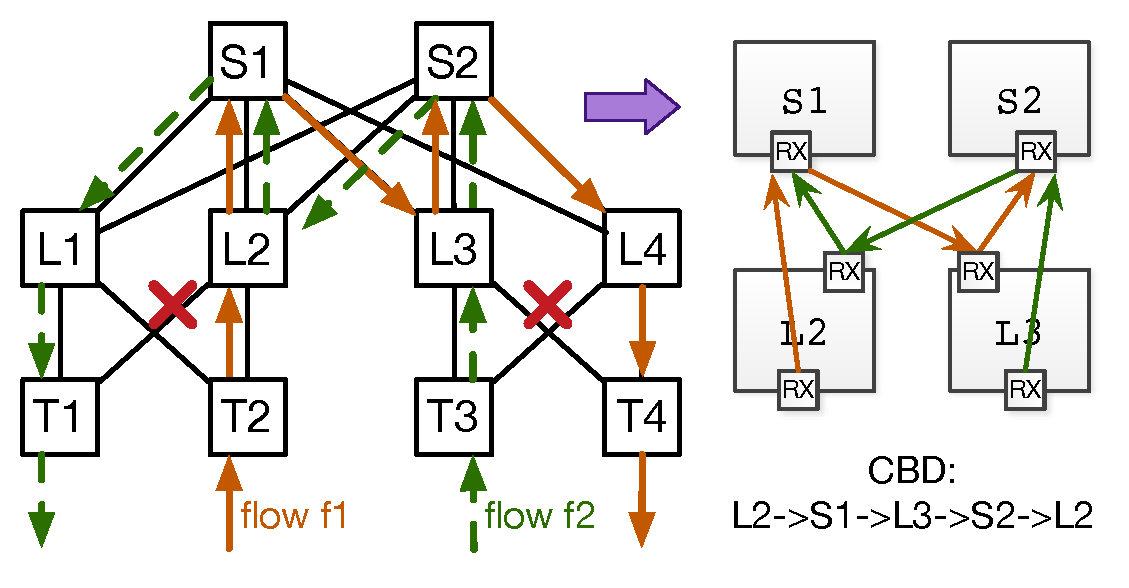
\includegraphics[width=0.5\textwidth] {figs/cbd_a}
	}
	
%	\vspace{-0.15in}
	\subfloat[short for lof][CBD is eliminated with path segmenting and prioritizing.]{
		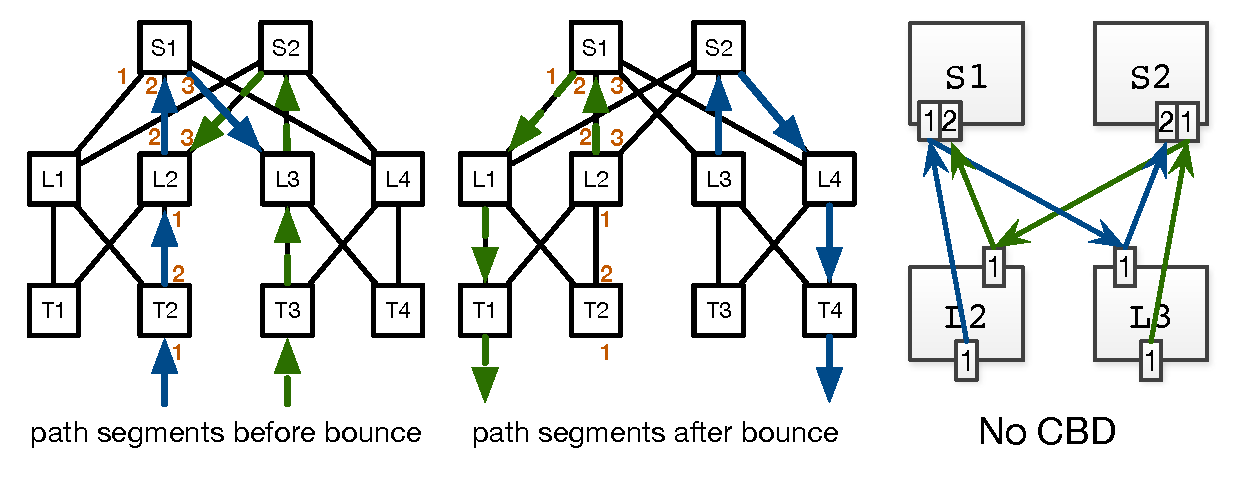
\includegraphics[width=0.5\textwidth] {figs/cbd_b}
	}
	
	\caption{Micropath based priority transition can eliminate CBD.}\label{fig:priority_transition}
\end{figure}

Figure~\ref{fig:priority_transition}(a) shows a simple Clos topology. Let's
assume that the operator wants all normal paths to be lossless. In addition,
let's assume that the operator is worried about rerouting due to link failures. 

Typically, the "normal" paths will be the shortest paths -- which for a CLOS
network are the ``up-down'' paths described in the last section.  In addition,
due to link failures, we may have paths that are not up-down.  Such paths can
form CBD, and lead to deadlock, as shown in
Figure~\ref{fig:priority_transition}(a))~\cite{shpiner2016unlocking}. 

However, if we divide the paths into two segments, {\em before-bounce} and {\em
after-bounce}, and assign them to different priority queues, there is no more
CBD (Figure~\ref{fig:priority_transition}(b)).  The insight we get from this
example is that if the switch can detect that a packet may cause CBD in next
hops, it can change the packet's priority to avoid CBD, thus avoiding deadlock. 

Note that this is different from the prior solutions, which either assign a
fixed priority based on pre-computed paths (and thus cannot react to dynamic
routing), or change the priority every hop (and thus requires too many priority
queues). 

Instead, we divide the paths into a few segments, which we call {\em micropaths},
and change packet's priority only at a few transition point. It has the
advantages from both types of prior work, {\em i.e.,} it requires a small number
of priorities, and allows the switch to react to each packet's path.

The key enabler of our approach is the topology and the set {\em lossless
routes} specified by the operators as the input. Specifying lossless routes is
not a significant burden: in our example, the operator may specify that all
normal up-down paths paths with a single ``bounce'' are ``lossless''. Given the
topology and the routing protocol it is easy to automatically enumerate all such
paths~\footnote{What happens if there are so many link failures that some
packets end up taking a two-bounce path? In such case, our tagging scheme moves
the packets to a lossy queue, which follows the standard drop-tail discipline.
Such queues, obviously, do not deadlock}. 

By properly dividing lossless routes into multiple subspaces of micropaths, we
can ensure that CBD is eliminated {\em within} each subspace. We will discuss
the details of the algorithm are described later in this section. But first, we
must consider another issue: Even though proper micropath partition ensures no
CBD {\em within} each priority, packets can still cause CBD {\em across}
priorities, as shown in Figure~\ref{fig:subspace}(a). Switch must know the past
path of each packet in order to decide the priority that avoids CBD. Obviously,
the tag size is limited, so we can't carry the entire history of the packet in
the tag. Thus, we need we need the next idea.

%% Section~\ref{sec:greedy} shows a way to achieve this.  Inevitably, we will need
%% {\em multiple} switch lossless queues to support one lossless application class.
%% Specifically, we divide the buffer of network nodes into $k$ partitions, and let
%% the $j$-$th$ partition associated with priority queue $j$. If a packet is
%% classified into priority queue $j$, it will be buffered in the $j$-$th$ buffer
%% partition and can generate PFC of priority $j$.  In this section, we focus on
%% supporting {\em just one} lossless application class. In
%% Section~\ref{sec:specific}, we will revisit this issue and show how we may
%% support multiple application classes more efficiently.

\subsection{Idea 2: Tag for Ordered Micropath Subspaces}\label{sec:tag_order}

\begin{figure}[t]
	%\vspace{-0.1in}
	\centering
	
	\subfloat[short for lof][CBD among subspaces.] {
		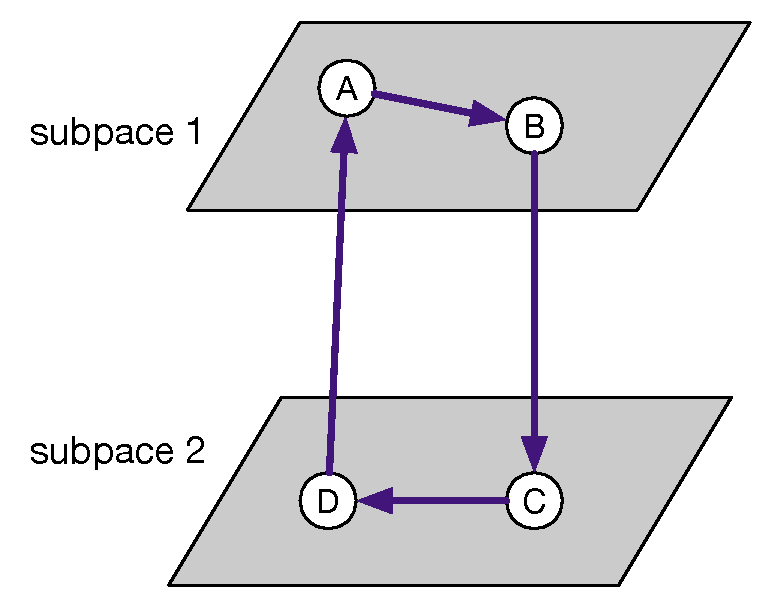
\includegraphics[width=0.24\textwidth] {figs/subspace_a}
	}
	\subfloat[short for lof][Ordered subspaces.]{
		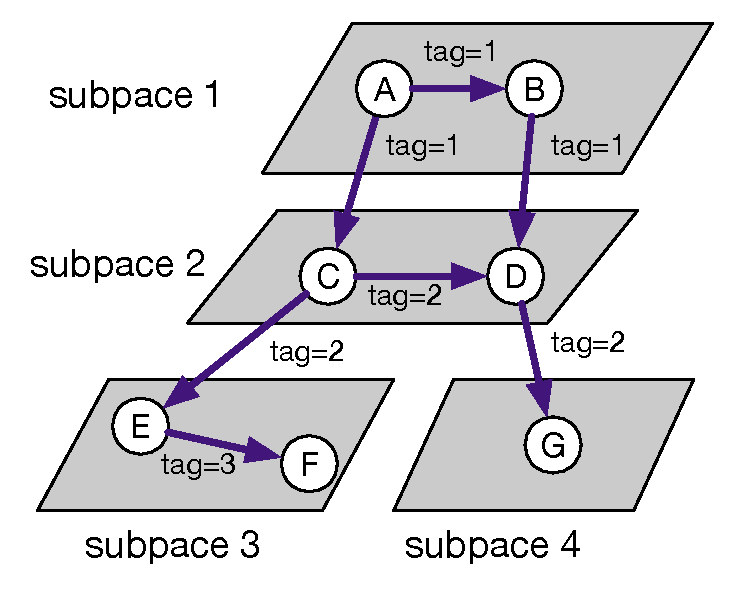
\includegraphics[width=0.26\textwidth] {figs/subspace_b}
	}
	
	\caption{Ordered subspaces ensure deadlock-free priority transition.}\label{fig:subspace}
\end{figure}

As shown in Figure~\ref{fig:subspace}(b), we enforce the order of transitioning
among micropath subspaces and tag only based on current subspace.  With this,
the packets do not need to record the whole history of past micropaths in
headers. A fixed length header field (most commonly, DSCP) is sufficient to
carry the tag. The tag values are one-one mapped to the micropath subspaces,
which one-one maps to priority queues on each switch. 

Thus, with \sysname{}, the switch enqueues each packet into priority queue based
on its tag, and changes the tag if the switch decides to change the packet's
priority at the next hop.  We can prove that the network is deadlock-free if the
tag system, which defines micropath subspaces and transition, satisfies the two
requirements below:

\begin{enumerate}

	\item A packet's tag is unchanged or changed at each hop of its path. When the tag is changed, it must be changed monotonically 
	along any packet's path (e.g., always increasing).

	\item For any given tag, all micropaths within the corresponding micropath subspace do not form cyclic buffer dependency.

\end{enumerate}

\para{Proof of deadlock freedom:}

\textbf{Claim:} Any tag system that satisfies the above two requirements is deadlock-free.

\textbf{Proof sketch:} We prove by contradiction. Suppose we can find a topology and a
set of lossless routes, for which there exists a subspace partition and priority
transition that satisfies the above two requirements, but is not deadlock-free.
Then, as the tag system is not deadlock-free, we can find a set of micropaths
that form a CBD. 

\textbf{Case 1:} All these micropaths are in the same subspace. According to
requirement 2, micropaths within the same subspace do not form CBD.
Contradicted.

\textbf{Case 2:} These micropaths are in different subspaces. We sort these
micropaths according to the subspaces they belong to, and choose a micropath in
the smallest subspace. Since these micropaths can form a CBD,  starting from the
source end of the chosen micropath, we can always find a circular path back to
the chosen micropath when traversing along these micropaths. 
 
According to requirement 1, once we enter a larger subspace, we can never go
back. So this circular path should only include micropaths in the smallest
subspace. But according to requirement 2, micropaths within the same subspace do
not form a CBD. Hence no circular path can be found within the smallest
subspace. So this circular path does not exist. Contradicted.
 
Thus, we conclude that there do not exist a set of micropaths that form a CBD.
This contradicts the supposition that the tag system is not deadlock-free.
Hence, any tag system that satisfies the above two requirements is
deadlock-free.

Putting these two ideas together we can generate a system of tags and tag
conversion tables for each switch. However, we must pay heed to the fact that 
a switch cannot support more than one or two lossless priorities in practice. 
Thus, we must minimize the number of tags we use.

\subsection{Idea 3: Minimizing the Number of Tags} The number of tags (or,
corresponding micropath subspaces) is essentially the number of lossless queues
required on each switch.  We must reduce it to below the switch hardware limit.
In this section, we focus on the number of lossless queues for just {\em one}
application class. We first formalize the tagging system.

\para{Tagging system.} Let $A_i$ represent a unique ingress port in the network, {\em i.e.,} switch $A$'s $i^{th}$ ingress port.
We use a {\em tagged graph} $G(V,E)$ to uniquely represent a tagging system.
With a tagging system, the {\em tagged graph} $G(V,E)$ is generated following below rules.

\begin{enumerate}
\item $G$ contains a node, $(A_i, x)$, {\em iff.} a port $A_i$ may receive packets with tag $x$, and these packets must 
be lossless. $V$ is the set of all such nodes.
\item In $G$, there exists an edge $(A_i, x)\rightarrow(B_j, y)$ {\em iff.} switch $A$ and $B$ are 
connected, {\em and} switch $A$ may change a packet's tag from $x$ to $y$ before sending to $B$ (the case $x=y$ also counts).
$E$ is the set of all such edges.
\end{enumerate}

The tags define a partition of the tagged graph, $\{G_k\}$, where $G_k = \{(A_i,
k) | \forall A, i\}$. Each $G_k$ is a {\em micropath subspace} and has a unique
lossless priority.  On switches, we configure ACL rules to match on tags and
assign lossless priorities.  In addition, each edge that has different tags on
two ends corresponds to an action of changing tags on switches.

Two requirements directly follow Section~\ref{sec:tag_order}. First, any $G_i$
does {\em not} have a cycle. This is because each edge in $G_i$ is essentially a
buffer dependency -- whether $A_i$ can dequeue packets depending on whether
$B_j$ has paused upstream. A cycle in $G_i$ means cyclic buffer dependency.
Second, There is no lossless route going from $G_i$ to $G_j$ if $i<j$, because
we enforce the order of micropath subspaces.


\para{Brute-force tagging system.} For general graph without structure information, a straight forward tagging system
to monotonically change the tag (thus, the priority) every hop, as described in Algorithm~\ref{alg:ttl}. It is easy to 
verify that the above requirements are met, so deadlock is eliminated with this tagging system. However, it requires 
too many lossless queues in a large network since it depends on the diameter of the topology.

\begin{algorithm}
	\small
    \KwIn{Topology and routing paths $R$ that must be lossless}
	\KwOut{A tagged graph $G(V, E)$}
	$V \gets Set()$\;
	$E \gets Set()$\; 
	$maxTag \gets$ longestPath($R$)\;
	\For{each path $r$ in $R$} {
		$tag \gets maxTag$\;
		\For{each hop $h$ in $r$} {
			$V \gets V \cup \{(h, tag)\}$\;
			$E \gets E \cup \{lastHop\rightarrow(h, tag)\}$\;
			$tag \gets tag-1$\;
		}
	}
	\Return{$G(V, E)$}\;
    \caption{A brute-force tagging system that decreases the tag by one every hop.}
	\label{alg:ttl}
\end{algorithm}

\begin{table}
\small
\centering
\begin{tabular}{|c|c|}
\hline
Symbol & Description \\ \hline
$A_i$ & Switch $A$'s $i^{th}$ ingress port  \\ \hline
$(A_i, x)$ & A node in tagged graph \\ \hline
$(A_i, x)\rightarrow(B_j, y)$ & A tagged edge \\ \hline
$V$ & All tagged nodes  \\ \hline
$E$ & All tagged edges \\ \hline
$G(V, E)$ & Tagged graph \\ \hline
\end{tabular}
\caption{Notations in the formalized description.}
\label{tab:symbols}
\end{table}

\para{Greedy algorithm.} Leveraging the brute-force tagging system as a start
point, we design Algorithm~\ref{alg:greedy} minize the number of lossless
queues. It works by greedily combining as many nodes, from brute-force tagging
system, as possible into each micropath subspaces under CBD-free constraint. To
ensure the monotonic property, we start from combing the nodes with largest tag
to smallest tag in the brute-force tagging system.  Obviously, the monotonic
property will still hold after combination. 

\begin{algorithm}
	\small
    \KwIn{The brute-force tagged graph $G(V, E)$}
	\KwOut{A new tagged graph $G'(V', E')$ that has small $|\{G'_k\}|$}
	$V' \gets Set()$\;
	$E' \gets Set()$\;
	$t' \gets 0$\;
	\For{$t \gets maxTag$ \textbf{down to} $minTag$} {
		$V_{tmp} \gets Set()$\;
		$E_{tmp} \gets Set()$\;
		\For{each $(A_i, t)$ in $V$ whose tag is $t$} {
			$V_{tmp} \gets V_{tmp} \cup \{A_i\}$\;
			$E_{tmp} \gets E_{tmp} \cup \{$edges whose both ends are in $V_{tmp}\}$\;
			\uIf{$G_{tmp}(V_{tmp}, E_{tmp})$ is acyclic} {
				$V' \gets V' \cup \{(A_i, t')\}$\;
				$E' \gets E' \cup \{$edges of $(A_i, t)$, change $t$ to $t'\}$\; 
			}
			\Else{
				$V' \gets V' \cup \{(A_i, t'+1)\}$\;
				$E' \gets E' \cup \{$edges of $(A_i, t)$, change $t$ to $t'+1\}$\;
			}
			$V \gets V \backslash \{v\}$ \;
		}
		\uIf{$V'$ contains nodes of tag $t'+1$} {
			$t' \gets t'+1$\;
		}
	}
	\Return{$G'(V', E')$}\;
    \caption{Greedily minimizing the number of micropath subspaces by merging brute-force tags.}
	\label{alg:greedy}
\end{algorithm}

We assign a new tag $t'$ (different from the brute-force tag) for each micropath
subspace, and generate switch configurations based on the algorithm output. The
worst case scenario is as bad as using the original input, brute-force tags,
which require as many priority queues as the length of longest lossless route.
However, in Section~\ref{sec:eval}, we show that this algorithm works reasonably
well for generic topology.  \fixme{highlight: For example, Jellyfish with 1000
nodes require only X priorities for {\em one} application class.}
